\chapter{Segmentazione di immagini}
\label{chapter_seg}
 La segmentazione è uno dei task più popolari nel campo del Deep Learning applicato alle immagini e, in generale, nel campo della Computer Vision. In particolare, consiste nel produrre una maschera delle stesse dimensioni dell'immagine in input, dove il valore di ogni pixel rappresenta la classe a cui è stato assegnato, o detto in altre parole, partizionare un'immagine in regioni con un valore semantico ben preciso (Figura \ref{fig:example_sem_seg}).

\begin{figure}[b!]
    \centering
    \hspace*{-0.1in}
    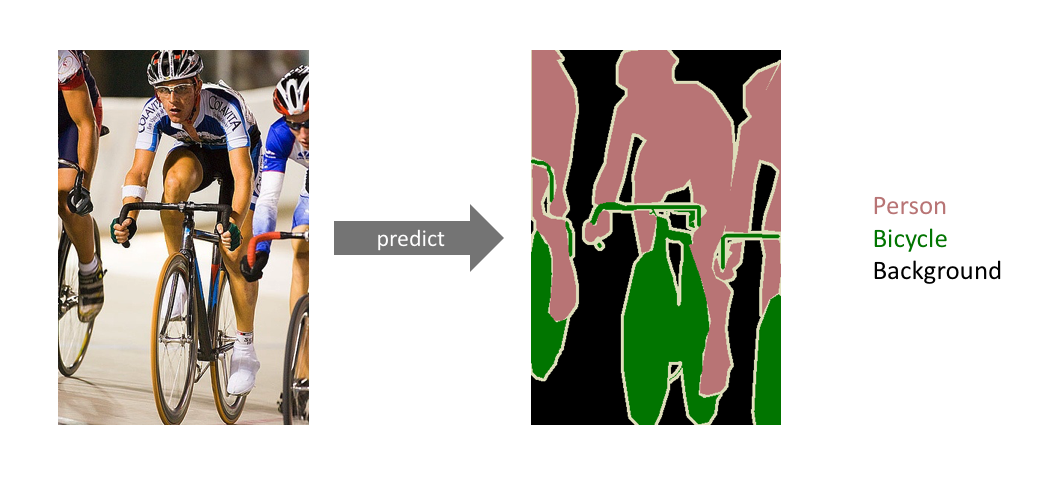
\includegraphics[scale=0.37]{img/example_sem_seg.png}
    \caption{Un esempio del risultato della segmentazione di un'immagine.}
    \label{fig:example_sem_seg}
\end{figure}

Grazie alle informazioni spaziali che si possono ottenere con la segmentazione, molti campi ne beneficiano, tra cui il campo dei veicoli autonomi, la detection di pedoni, diagnosi medica assistita da computer e molti altri \cite{semsegsurvey}. 

%Grazie al fatto che la segmentazione permette di ottenere sull'immagine in input, oltre che informazioni semantiche, anche informazioni spaziali, molti campi ne beneficiano, tra cui, il campo dei veicoli autonomi, la detection di pedoni, diagnosi medica assistita da computer e molti altri \cite{semsegsurvey}. 

%\subsubsection{Tipi di immagini}
In letteratura la segmentazione è stata applicata a una grande varietà di dati. Alcune tra le tipologie più utilizzate sono: 
\begin{itemize}
    \item \textbf{scala di grigi}: un tipo di immagine che presenta un solo canale e il valore dei pixel rappresentano, sostanzialmente, la quantità di luce del pixel.
    
    \item \textbf{RGB (red, green and blue)}: probabilmente la tipologia più nota, presenta tre canali che rappresentano rispettivamente la quantità di rosso, di verde e di blu del pixel.
    
    \item \textbf{RGB-D}: un tipo di immagine che, oltre ad avere i tre canali del RGB, ha anche un quarto canale che rappresenta la profondità di quel pixel, ovvero la distanza dalla camera, informazione spesso molto utile nel campo della segmentazione semantica \cite{qi20173d}.
    
    \item \textbf{3D}: un tipo di dato spesso presente nella letteratura medica, come ad esempio nel campo della TC (tomografia computerizzata), dove le immagini vengono catturate con strumenti a raggi X \cite{hu2001automatic}.
\end{itemize}
%\subsubsection{Dataset di benchmark}
Come detto in precedenza, la segmentazione è uno dei task più popolari e negli anni nel campo della ricerca, sono stati fatti molti passi avanti, sviluppando modelli e algoritmi sempre più performanti. In particolare, le performance di questi modelli sono state misurate testandoli su dei dataset, che sono stati usati come benchmark per paragonare i vari metodi. Tra i dataset di benchmark più noti ed utilizzati ci sono:
\begin{itemize}
    \item \textbf{PASCAL-VOC} (PASCAL Visual Object Classes) \cite{pascal-voc}
    \item \textbf{Cityscapes dataset} \cite{cityscapes}
    \item \textbf{ADE20K} \cite{zhou2019semantic}
\end{itemize}
Nel campo della computer vision, la segmentazione viene affrontata con diversi metodi. In particolare, esistono metodi tradizionali, che non fanno uso di tecniche di Machine Learning; metodi di Machine Learning; e infine metodi di Deep Learning, che sfruttano invece architetture che, come vedremo più avanti, riescono ad apprendere pattern molto complessi che i metodi tradizionali e di Machine Learning spesso non riescono a cogliere.
Per quanto riguarda i metodi tradizionali, le tecniche sono svariate: alcune sono basate sull'estrazione di feature e altre sul preprocessing dell'immagine in input; invece, per quanto riguarda i metodi di Machine Learning, essi sono basati sul trasformare i pixel dell'immagine in una rappresentazione che poi può essere utilizzata dagli svariati algoritmi di Machine Learning per classificarli, come il K-Means o l'SVM (Support Vector Machines). Invece, le architetture di Deep Learning sono diverse e tra le più utilizzate ci sono la UNet\cite{unet}, la DeepLabV3\cite{deeplabv3}, la PSPNet\cite{pspnet}, la FCN\cite{FCNs} e altre. Vedremo più avanti i concetti di Deep Learning sui quali si basano queste architetture.
Al di là delle metodologie utilizzate, un aspetto molto importante dello sviluppare un algoritmo, un'architettura, oppure utilizzarne una già esistente, consiste nella scelta della metrica di valutazione. Di metriche ne esistono diverse:

\begin{itemize}
    \item \textbf{Accuracy}: questa è probabilmente la più semplice e più intuitiva, ovvero misura il numero di pixel correttamente classificati, chiaramente in proporzione al numero totale di pixel. Questa metrica è generalmente una delle più utilizzate nel campo del Machine Learning.
    Viene definita come:
    
    \begin{equation}
        Accuracy = \frac{\sum_{i=1}^k{n_{ii}}}{\sum_{i=1}^k{t_{i}}}.
    \end{equation}
    
    Dove $k$ è il numero di classi, $n_{ij}$ è il numero di pixel di classe $i$ e classificati come di classe $j$ e $t_{i}$ il numero totale di pixel della classe $i$ ovvero:
    
    \begin{equation}
        t_{i} = \sum_{j=1}^k{n_{ij}}.
    \end{equation}
    Inoltre, a parte l'accuracy generale, che in pratica misura l'accuratezza del modello, ma non facendo caso alle singole classi, possiamo anche utilizzare l'accuracy di una classe. In particolare, l'accuracy di una singola classe $i$ è definita come il rapporto tra il numero di pixel di quella classe correttamente classificati dal modello e il numero totale di pixel di quella classe:
    
    \begin{equation}
        Accuracy_{i} = \frac{n_{ii}}{t_{i}}.
    \end{equation}
    
    Il principale svantaggio nell'utilizzo dell'accuracy è che in molti task alcune classi prevalgono rispetto alle altre, di conseguenza utilizzare l'accuracy può portare ad avere un valore alto, ma che in realtà è causato dalla predominanza di quella classe. Ad esempio, se in un'immagine l'80\% dei pixel è di una classe, un modello che classifica tutti i pixel dell'immagine come appartenente a quella classe, otterrebbe una accuracy dell'80\%.
    
    
    \item \textbf{Accuracy media}: questa ed altre metriche fanno fronte al problema sopra menzionato dell'accuracy. Questa metrica, in particolare, rappresenta la media delle accuracy delle singole classi e risolve il problema normalizzando l'accuracy rispetto al numero totale dei pixel:
    
    \begin{equation}
        MeanAccuracy = \frac{1}{k} \sum_{i=1}^k{Accuracy_{i}} = \frac{1}{k} \sum_{i=1}^k{\frac{n_{ii}}{t_{i}}}.
    \end{equation}
    
    
    \item \textbf{Mean intersection over union (mIoU)}: anche chiamato \textit{Jaccard index}, è la media dell'\textit{intersection over union (IoU)} dell $k$ classi, dove l'IoU di una classe è essenzialmente il rapporto tra l'intersezione e l'unione di due insiemi: l'insieme dei pixel di quella classe nella maschera e l'insieme dei pixel di quella classe nella predizione, ovvero:
    
    \begin{equation}
        IoU = \frac{target \cap prediction}{target \cup prediction}.
    \end{equation}
    
    definibile anche come
    
    \begin{equation}
        IoU = \frac{n_{ii}}{t_{i}-n_{ii}+\sum_{j=1}^k{n_{ij}}}.
    \end{equation}
    
     e di conseguenza la mIoU è definita come:
     
     \begin{equation}
         mIoU = \frac{1}{k} \sum_{i=1}^k{IoU_{i}} =
         \frac{1}{k} \sum_{i=1}^k{\frac{n_{ii}}{t_{i}-n_{ii}+\sum_{j=1}^k{n_{ij}}}}.
     \end{equation}
     
     
    \item \textbf{Frequency weighted intersection over union (FWIoU)}: una variante della mIoU, che invece di calcolare semplicemente la media delle IoU, calcola una media pesata rispetto al numero di pixel delle classi (frequenza), ovvero:
    
    \begin{equation}
        FWIoU = (\sum_{i=1}^k{t_{i}})^{-1} \sum_{i=1}^k{t_{i}IoU_{i}} = (\sum_{i=1}^k{t_{i}})^{-1} \sum_{i=1}^k{t_{i}\frac{n_{ii}}{t_{i}-n_{ii}+\sum_{j=1}^k{n_{ij}}}}.
    \end{equation}
    
    
    \item\textbf{Matrice di confusione}: non è una vera e propria metrica, ma è un metodo molto utilizzato anche e soprattutto nel campo della classificazione. La matrice di confusione è molto utile in particolare quando si vuole approfondire la natura degli errori del proprio metodo. Nello specifico, ci mostra per ogni classe $i$ il numero di pixel correttamente predetti $n_{ii}$ ma, ancora più importante, per ogni classe ci mostra la suddivione degli errori nelle altre classi, ovvero $n_{ij}$ per $j \in [1,2,..., i-1, i+1, ..., k]$. Di conseguenza, possiamo rappresentare formalmente la matrice di confusione come:
    
    \begin{equation}
        ConfusionMatrix = [n_{ij}].
    \end{equation}
    
    dove  $i,j \in [1, 2, ..., k]$.
    
\end{itemize}

Inoltre, nel campo della Computer Vision, così come nel mondo algoritmico, i metodi vengono valutati secondo due ulteriori criteri: la complessità temporale, molto importante soprattutto in alcuni campi di applicazione dove il tempo necessario per processare un'immagine e produrre la sua segmentazione non deve essere maggiore di una certa soglia, come il campo dei veicoli autonomi; e la complessità spaziale, ovvero la quantità di memoria di cui ha bisogno l'algoritmo, metrica molto importante soprattutto in campi dove il processamento avviene su dispositivi che non abbondano di memoria, come smartphones e fotocamere.












\section{La segmentazione di immagini negli umani}
Partendo da come gli umani percepiscono un'immagine e riescono naturalmente e in modo intuitivo a segmentarla, il funzionamento di tali intuizioni si basa su quella che è chiamata "psicologia della Gestalt" \cite{gestalt} (dal tedesco \textit{Gestaltpsychologie}, 'psicologia della forma' o 'rappresentazione'). La piscologia della Gestalt spiega come un umano riesca a percepire un'immagine e organizzarla in un sistema complesso. In particolare, spiega come, guardando il mondo intorno a sé, riesca a percepire scene complesse composte da molti gruppi di oggetti su uno sfondo, che a loro volta possono essere costituiti da altre parti e via dicendo.
Il modo in cui gli umani riescano a raggiungere un risultato percettivo così notevole, visto il fatto che l'input visivo è, in un certo senso, solo una distribuzione spaziale di punti individuali variamente colorati, è basato su dei principi che definiscono le intuizioni dietro il raggruppamento di parti dell'immagine. Non esiste una lista precisa dei principi della Gestalt, ma ne esistono alcuni che sono più discussi e più comunemente utilizzati \cite{todorovic2008gestalt}:

\begin{itemize}
    \item \textbf{principio di buona forma}: la struttura di oggetti che tendiamo a percepire è sempre la più semplice.

    \item \textbf{principio di prossimità}: formalizza l'intuizione dietro il fatto che tendiamo a raggruppare elementi vicini tra loro.
    
    \item \textbf{principio di destino comune}: tendenza a raggruppare elementi che hanno un movimento coerente tra loro.
    
    \item \textbf{principio di somiglianza}: tendenza a raggruppare gli elementi simili tra loro (in colore, forma, grandezza, ...)
    
    \item \textbf{principio di buona continuità}: tendenza a raggruppare elementi per formare oggetti e forme continue e coerenti nello spazio.
    
    \item \textbf{principio dell'esperienza passata}: l'osservatore tende a raggruppare gli elementi visivi in modo coerente al modo in cui li ha visti nel suo passato.
\end{itemize}

In generale, questi principi formalizzano delle intuizioni comuni alla piscologia di tutti gli umani. Il problema è che queste intuizioni sono spesso molto difficili da trasformare in un linguaggio matematico o in un algoritmo, e da qui nasce la difficoltà della segmentazione e di altri task nel campo della Computer Vision, che come quest'ultima risultano spesso intuitivi, ma molto difficili da trasformare in un algoritmo.
Inoltre, anche per gli umani, a volte, il task della segmentazione risulta complesso e i risultati, quando cambia il soggetto, sono spesso diversi tra loro.  Questo ci fornisce un'intuizione di come, a differenza di altri task come la classificazione, il problema della segmentazione sia particolarmente difficile anche solo da definire \cite{martin2001database}.







\section{Approcci classici}
Come detto in precedenza, il task della segmentazione d'immagini può essere affrontato con diversi approcci classici. Alcuni di questi trasformano il task in un problema di ottimizzazione, cercando poi di risolverlo con algorimi iterativi,  altri invece lo trasformano in un problema di \textit{clustering}, trasportando l'immagine in uno spazio a più dimensioni per poi utilizzare algoritmi di Machine Learning. 







\subsection{Metodi a soglia}
\label{metodi_soglia}
Uno dei metodi più semplici e intuitivi è il metodo a soglia (\textit{thresholding}). In pratica, esso consiste nel definire una soglia numerica di una feature dell'immagine, per poi classificare i pixel in base a questa soglia. Nella sua forma più semplice, definendo un'unica soglia l'immagine viene segmentata in due classi; nella sua variante multiclasse, invece, si definiscono più soglie, creando così degli intervalli che rappresentano le diverse classi. La feature utilizzata più spesso è quella dell'intensità dei pixel (in immagini in scala di grigi), ma se ne possono utilizzare tante altre, questo dipende molto dal campo di applicazione e dalla natura dell'immagine. Ad esempio, una feature spesso molto utile per segmentare un'immagine è la profondità. Il problema principale consiste nel fatto che questo tipo di feature, a parte il caso in cui sia fornito direttamente dall'immagine (RGB-D), è spesso molto difficile da estrarre.
Chiaramente, questo metodo restituisce spesso risultati approssimativi e inoltre la ricerca del valore ottimale della soglia non è affatto semplice e richiede spesso un'approfondita conoscenza del dominio.





\subsection{Metodi dividi e fondi}
\label{metodi_dividi_fondi}
Come abbiamo visto nel paragrafo precedente, una delle tecniche più semplici è definire una soglia con cui classificare i pixel. Sfortunatamente, nella maggior parte dei casi trovare questa soglia è molto difficile e molto spesso non è nemmeno unica, ovvero le immagini a volte presentano forti differenze da una regione all'altra, di conseguenza una buona soglia per una parte può risultare non buona per un'altra. 
Data questa difficoltà, una tecnica per risolverla consiste nel suddividere l'immagine in parti diverse oppure, al contrario, cercare di unire parti di immagine simili tra loro.
Uno dei primi algoritmi che rientra in questa categoria è l'algoritmo degli spartiacque (in inglese \textit{watershed}) \cite{watershed}, che considera le immagini in scala di grigi come una mappa topografica, trasformando l'intensità dei pixel nell'altezza. In particolare, utilizzando la metafora di un'alluvione, l'algoritmo suddivide l'immagine in diversi bacini idrografici, ovvero le regioni segmentate delle immagini sono composte da tutti quei punti da cui l'acqua finirebbe nello stesso punto (il minimo) (Figura \ref{fig:watershed}). Sfortunatamente, anche questo algoritmo spesso restituisce risultati approssimativi, in particolare, uno dei maggiori problemi è che, associando una regione ad ogni minimo locale, spesso over-segmenta l'immagine. Infatti, questo algoritmo è soprattutto usato in sistemi interattivi dove la segmentazione è assistita da un utente che definisce il centro degli oggetti d'interesse.
\\ \\
\begin{figure}[h!]
    \centering
    \hspace*{-0.1in}
    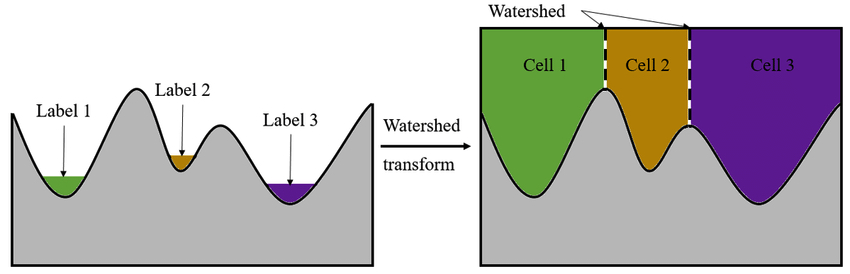
\includegraphics[scale=0.4]{img/watershed2.jpg}
    \caption{Illustrazione di come l'algoritmo degli spartiacque trova le soglie (watershed nell'immagine) con cui segmentare le immagini.}
    \label{fig:watershed}
\end{figure}

Infine, ci sono altri metodi che, invece che cercare di suddividere l'immagine in regioni, cercano al contrario di unire tra loro regioni che abbiano una certa similarità con un approccio \textit{bottom-up}. Una categoria di questi sono i metodi basati su grafi.




\subsection{Metodi basati su grafi}
\label{metodi_grafi}
Questa categoria di metodi si basa sulla rappresentazione dell'immagine come un grafo $G=(V,E)$ dove i vertici $V$ sono i pixel e gli archi $E$ sono tra i pixel adiacenti. Uno degli algoritmi che fa parte di questa categoria è quello proposto in \cite{graph_segm}, in cui i pesi rappresentano una misura di dissimilarità tra i pixel che connettono. Questa misura di dissimilarità $w(e)$ può prendere diverse forme e quella più semplice è probabilmente la differenza di intensità tra i due pixel. 
Una qualsiasi regione $R$ ha una misura di differenza interna chiamata $Int(R)$, che è definita come il massimo peso di un arco all'interno dell'albero ricoprente minimo di $R$, ovvero $MST(R)$: 

\begin{equation}
    Int(R) = \max_{e\in MST(R)} w(e).
\end{equation}

Inoltre, per due regioni adiacenti, ovvero che hanno minimo un arco che le connette, si definisce la differenza tra loro come il peso minimo di un arco che le connette:

\begin{equation}
    Dif(R_{1}, R_{2}) = \min_{e=(v_{1}, v_{2}) | v_{1} \in R_{1}, v_{2} \in R_{2}} w(e).
\end{equation}

L'algoritmo unisce iterativamente tra loro due qualsiasi regioni $R_{1}$ e $R_{2}$ se la loro differenza $Dif(R_{1}, R_{2})$ è minore della minima differenza interna delle due regioni $MInt(R_{1}, R_{2})$, dove

\begin{equation}
    MInt(R_{1}, R_{2}) = min(Int(R_{1}) + \tau(R_{1}),  Int(R_{2}) + \tau(R_{1})).
\end{equation}

Dove $\tau(R_{1})$ rappresenta quanto la differenza tra le due regioni debba essere più grande delle differenze interne per non essere fuse, ma segmentate in due regioni diverse, ed è definito come:

\begin{equation}
    \tau(R) = \frac{k}{|R|}.
\end{equation}

Dove $k$ è un paramtero costante e $|R|$ è la dimensione della regione. In realtà, questo componente $\tau$ può assumere diverse forme a seconda dello specifico task e in base a come si voglia definire la bontà di una regione.
Infine, la regola con cui l'algoritmo decide iterativamente di unire o meno due regioni è la seguente: unire $R_{1}$ e $R_{2}$ se $Dif(R_{1}, R_{2})<MInt(R_{1}, R_{2})$.
\\ \\
\begin{figure}[h!]
    \centering
    \hspace*{-0in}
    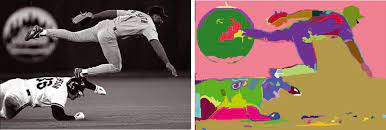
\includegraphics[scale=1]{img/graph_segm.jpeg}
    \caption{Esempio del risultato dell'algoritmo basato su grafi proposto in \cite{graph_segm} applicato su un'immagine in scala di grigi.}
    \label{fig:graph_baseball}
\end{figure}




\subsubsection{Tagli normalizzati}
Un altro algoritmo molto popolare che appartiene a questa categoria è quello proprosto in \cite{shi2000normalized}. In questo algoritmo, il peso di un arco $w_{i,j}$ tra i due pixel $i$ e $j$ rappresenta la loro affinità. L'idea dietro l'algoritmo è partizionare il grafo in regioni che abbiano affinità deboli, ovvero regioni connesse da archi con pesi bassi. Per definire il costo di un taglio tra due regioni $A$ e $B$, viene definita la seguente misura:

\begin{equation}
    cut(A, B) = \sum_{i \in A, j \in B}{w_{i,j}}.
\end{equation}

Definito questo costo, non basta che trovare i tagli che lo minimizzino. Il problema è che utilizzando solamente questo costo, i tagli risultanti sono normalmente quelli che isolano singoli pixel, di conseguenza va aggiunto al costo un altro componente che penalizzi i sottografi piccoli.
Una migliore misura del costo di un taglio è la seguente misura, ovvero il costo del taglio normalizzato rispetto all'associazione dei due sottografi:

\begin{equation}
    NCut(A,B) = \frac{cut(A,B)}{assoc(A,V)} + \frac{cut(A,B)}{assoc(B,V)}.
\end{equation}

Dove $assoc(A,V)= \sum_{u \in A, t \in V}{w_{ut}}$ ovvero la somma dei pesi degli archi tra i nodi $A$ e tutti i nodi del grafo totale $V$ (compresi anche quelli $A$ stesso). In questo modo, normalizzando il costo rispetto all'associazione, penalizziamo i sottografi molto piccoli. Purtroppo però, la difficoltà di questo algoritmo sta nel fatto che minimizzare $NCut$ è un problema NP-completo.











\subsection{Metodo dei contorni attivi}
\label{metodi_contorni}
A volte, il task della segmentazione viene trasformato nel task della detection delle frontiere degli oggetti, ovvero dei loro bordi. In questo contesto vengono utilizzati i contorni attivi (\textit{active contours)}, anche detti \textit{snakes} (per la loro forma), che non sono altro che delle curve che, iterativamente, si vanno a stringere intorno ad un oggetto, prendendo mano a mano la sua forma fino a che, auspicabilmente, non la eguaglino alla perfezione. Questo tipo di metodo è spesso molto utile in contesti dove, ad esempio, sia necessario tracciare la forma di un oggetto in un video o di un oggetto che cambi prospettiva; il motivo è che le performance di questo metodo dipendono molto dall'inizializzazione della curva. In particolare, quando la curva viene inizializzata con una certa forma e abbastanza vicino all'oggetto, si hanno più probabilità di ottenere una segmentazione più precisa. Ad esempio, se in un video l'algoritmo è riuscito a segmentare l'oggetto del frame precedente, oppure quest'ultimo è stato segmentato a mano dall'utente, quel contorno, salvo grandi cambiamenti, è un'ottima inizializzazione per il frame successivo (Figura \ref{fig:lip_track}).

\begin{figure}[h!]
    \centering
    \hspace*{-0in}
    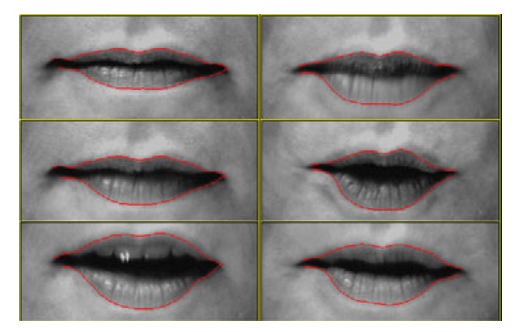
\includegraphics[scale=0.6]{img/active-cont.png}
    \caption{Esempio di applicazione dei contorni attivi: lip tracking.}
    \label{fig:lip_track}
\end{figure}

Questo tipo di algoritmo si basa su informazioni locali del gradiente dell'intensità dei pixel e le utilizza per attrarre la curva verso i bordi dell'oggetto. In particolare i bordi, essendo caratterizzati da un cambiamento improvviso dell'intensità, presentano un gradiente elevato, di conseguenza l'algoritmo cerca iterativamente di portare i punti che formano la curva in pixel con gradienti alti.
Questo meccanismo viene formalizzato con un problema di ottimizzazione, ovvero si vuole massimizzare la somma dei gradienti dell'intensità dei pixel dove sono i punti della curva.
Per quanto riguarda la definizione di un contorno, esso è definito come un insieme di punti nello spazio bidimensionale connessi da linee rette:

\begin{equation}
    V = \{v_{i} = (x_{i}, y_{i}) | i = 0,1,2,...., n-1\}.
\end{equation}

Dove $n$ è il numero dei punti che formano la curva. Come detto precedentemente, si vuole massimizzare la somma dell'intensità dei gradienti e per fare ciò viene utilizzata la magnitudine del gradiente dell'intensità dei pixel al quadrato, ovvero $||\nabla I||^{2}$. Inoltre, dato che la curva deve essere attratta dai gradienti più alti, bisogna espandere il "campo di forza" dei picchi del gradiente, altrimenti un punto non vicinissimo a un bordo non verrebbe attratto. Per fare questo utilizziamo la sfocatura gaussiana applicata alla magnitudine del gradiente e di conseguenza il valore da massimizzare diventa $||\nabla n_{\sigma} \ast I||^{2}$. Infine, il problema viene trasformato nel trovare il minimo di $E_{image}$, dove:

\begin{equation}
    E_{image} = -\sum_{i=0}^{n-1}{||\nabla n_{\sigma} \ast I(v_{i})||^{2}}.
\end{equation}

A questo punto, l'algoritmo non fa altro che cercare iterativamente di ottimizzare $E_{image}$ portando ogni punto in una nuova posizione, fino a che questo non raggiunge una certa soglia stabilita in anticipo. Il problema di questa versione è che è molto sensibile al rumore e molto spesso il contorno tende ad assumere forme strane, proprio a causa della presenza del rumore del gradiente intorno all'oggetto. 
Per superare questa difficoltà, e perché in generale si vuole una curva che rispetti alcune caratteristiche naturali, come se simulasse un oggetto fisico, come l'elasticità e la morbidezza, al problema di ottimizzazione viene aggiunto un secondo componente $E_{contour}$ che rappresenta questi vincoli di forma.
In particolare, $E_{contour}$ è composta a sua volta da altri due componenti $E_{elastic}$ e $E_{smooth}$, che rappresentano le due caratteristiche appena menzionate. In realtà, a $E_{contour}$ possono essere aggiunti altri componenti a seconda del task specifico e di come si voglia vincolare la forma della curva. Ad esempio, molto spesso quando si conosce a priori la forma dell'oggetto d'interesse, si può aggiungere al problema un componente che penalizzi forme diverse da questa. Di conseguenza, la formula di $E_{contour}$ è la seguente:

\begin{equation}
    E_{contour} = \alpha E_{elastic} + \beta E_{smooth}.
\end{equation}

Dove $\alpha$ e $\beta$ sono due coefficienti che rappresentano il peso che vogliamo dare ai due vincoli di elasticità e morbidezza.
Per quanto riguarda il vincolo di elasticità, esso rappresenta il desiderio che la curva simuli il comportamento di un elastico, ovvero quando due punti della curva sono più distanti c'è una sorta di forza di attrazione più forte e di conseguenza la curva tende a non distanziare troppo i punti tra loro. Di seguito la formula del componente di elasticità di un punto del contorno $v(s)$.

\begin{equation}
    E_{elastic}(v(s)) = \bigg|  \frac{\delta}{\delta s} v(s)  \bigg|^{2}.
\end{equation}


Ovvero il quadrato della derivata prima del punto del contorno, che rappresenta l'intuizione del fatto che non si vogliono grandi distanze da un punto all'altro. Per quanto riguarda il componete di morbidezza, invece, esso è definito come:


\begin{equation}
    E_{smooth}(v(s)) = \bigg|  \frac{\delta^{2}}{\delta^{2} s} v(s)  \bigg|^{2}.
\end{equation}

Ovvero il quadrato della derivata seconda del punto del contorno, che invece rappresenta l'intuizione del fatto che non si vogliono cambiamenti improvvisi. Dato che in realtà la curva del contorno è composta da punti discreti, le formule dei due componenti diventano:


\begin{equation}
    E_{elastic}(v(i)) = (x_{i+1} - x_{i})^{2} + (y_{i+1} - y_{i})^{2}.
\end{equation}

\begin{equation}
    E_{smooth}(v(i)) = (x_{i+1} -  2x_{i} + x_{i-1})^{2} + (y_{i+1} -  2y_{i} + y_{i-1})^{2}.
\end{equation}

e quindi

\begin{equation}
    E_{elastic} = \sum_{i=0}^{n-1}{(x_{i+1} - x_{i})^{2} + (y_{i+1} - y_{i})^{2}}.
\end{equation}

\begin{equation}
    E_{smooth} = \sum_{i=0}^{n-1}{(x_{i+1} -  2x_{i} + x_{i-1})^{2} + (y_{i+1} -  2y_{i} + y_{i-1})^{2}}.
\end{equation}


Infine, il problema totale diventa minimizzare il seguente valore:

\begin{equation}
    E_{total} = E_{image} + E_{contour}.
\end{equation}

La Figura \ref{fig:coin-contour} illustra un esempio di come il risultato migliori aggiungendo il componente $E_{contour}$.
\\
\begin{figure}[h!]
    \centering
    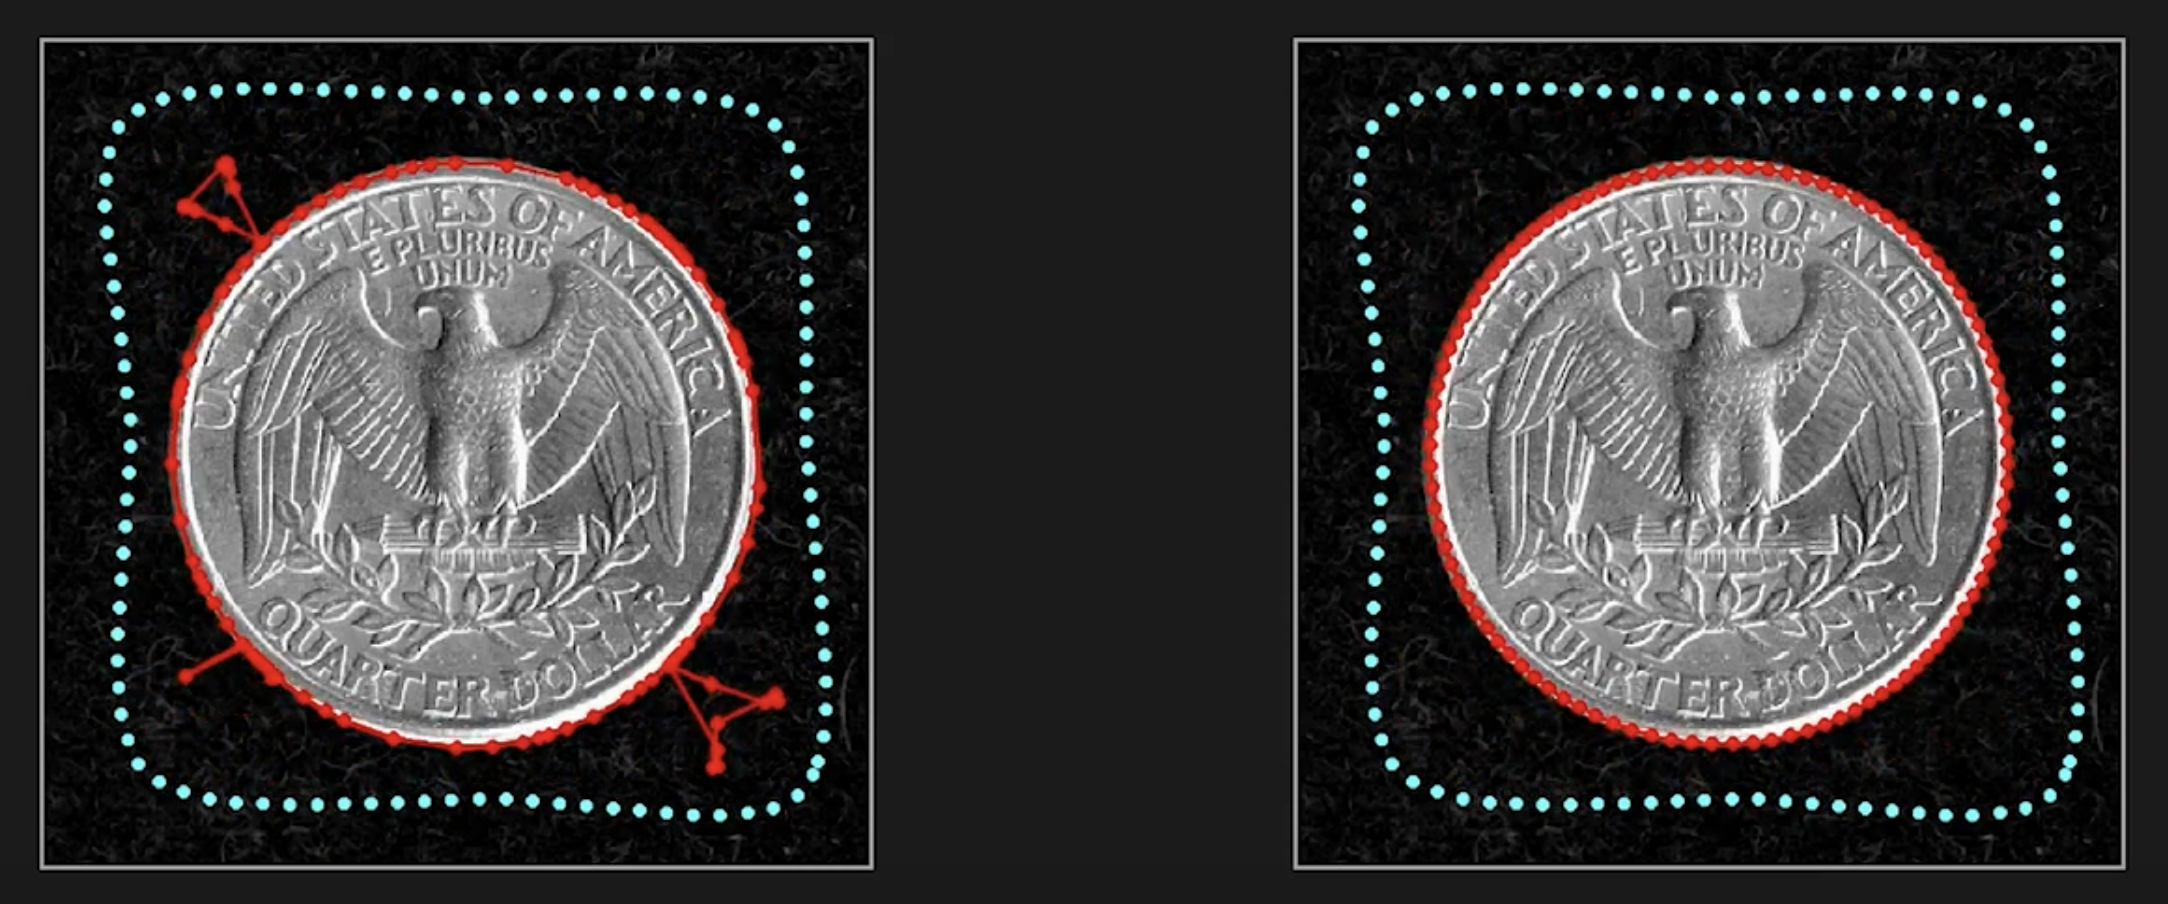
\includegraphics[scale=0.35]{img/activ_cont3.png}
    \caption{Esempio di applicazione del metodo del contorno attivo. In entrambe le immagini possiamo vedere un contorno blu (contorno di inizializzazione) e uno rosso (contorno finale). In particolare, a sinistra è stata utilizzata la versione dell'algoritmo che minimizza $E_{image}$, mentre a destra viene minizzato $E_{total}$ e possiamo notare come quello a destra ottenga un risultato migliore.}
    \label{fig:coin-contour}
\end{figure}

Come già anticipato, le performance di questo algoritmo dipendono molto dalla bontà dell'inizializzazione, inoltre performa bene soprattutto con immagini che contengono un solo oggetto, anche se si può utilizzare su immagini che ne contengono più di uno. In particolare, a seconda della natura degli oggetti si possono variare i parametri $\alpha$ e $\beta$, per dar modo al contorno di adattarsi meglio  agli oggetti (Figura \ref{fig:two-coin-segm}). In altri casi, come già menzionato, può risultare utile aggiungere ulteriori componenti a $E_{contour}$ oltre a $E_{elastic}$ e $E_{smooth}$.
Infine, esiste una variante dell'algoritmo che, invece di far partire il contorno da una forma più larga per poi farlo contrarre sull'oggetto, fa partire il contorno dal suo interno e lo fa gonfiare fino a modellare i suoi bordi.

\begin{figure}
     \centering
     \begin{subfigure}[b]{0.6\textwidth}
         \centering
         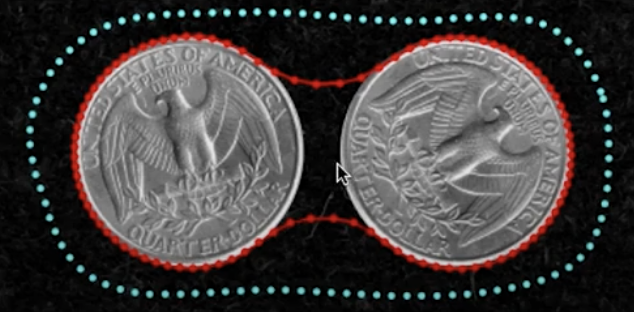
\includegraphics[width=\textwidth]{img/activ_cont4.png}
         \caption{$\alpha$ piccolo}
         \label{fig:y equals x}
     \end{subfigure}
     \hfill
     \begin{subfigure}[b]{0.6\textwidth}
         \centering
         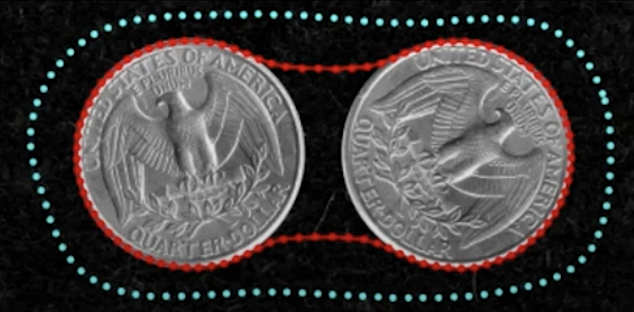
\includegraphics[width=\textwidth]{img/activ_cont5.png}
         \caption{$\alpha$ grande}
         \label{fig:three sin x}
     \end{subfigure}
        \caption{Esempio di segmentazione di due oggetti con un contorno attivo, variando però il coefficiente $\alpha$. Come si può notare, abbassando $\alpha$ si dà modo al contorno di adattarsi meglio ai due oggetti. Chiaramente, come modificare i due coefficienti $\alpha$ e $\beta$ dipende dalla natura dell'immagine.}
        \label{fig:two-coin-segm}
\end{figure}











\subsection{Metodi di clustering}
\label{metodi_clustering}
Così come i metodi basati su grafi hanno trasformato l'immagine in un grafo facendo corrispondere a ogni pixel un nodo, allo stesso modo i metodi di clustering trasformano l'immagine in una distribuzione in uno spazio euclideo a più dimensioni. In particolare, la prima fase di un metodo di questa categoria è capire su quali feature basarsi per mappare ogni pixel in un punto dello spazio. Una delle scelte più semplici, nel caso di immagini RGB, è quella di utilizzare i tre canali dell'immagine, ovvero la quantità di rosso, di verde e di blu (Figura \ref{fig:scimmia}). Altre feature molto utilizzate sono la luminosità, la posizione del pixel, la profondità (RGB-D), ma anche feature più complesse come la texture. Ancora una volta, la scelta di queste feature è molto importante, ma soprattutto dipende fortemente dal campo di applicazione e dalla natura delle immagini, di conseguenza è necessaria un'approfondita conoscenza di entrambi.

\begin{figure}[h!]
     \centering
     \begin{subfigure}[b]{0.4\textwidth}
         \centering
         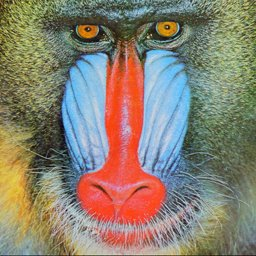
\includegraphics[width=\textwidth]{img/scimmia.jpeg}
         \caption{}
         \label{fig:y equals x}
     \end{subfigure}
     \hfill
     \begin{subfigure}[b]{0.5\textwidth}
         \centering
         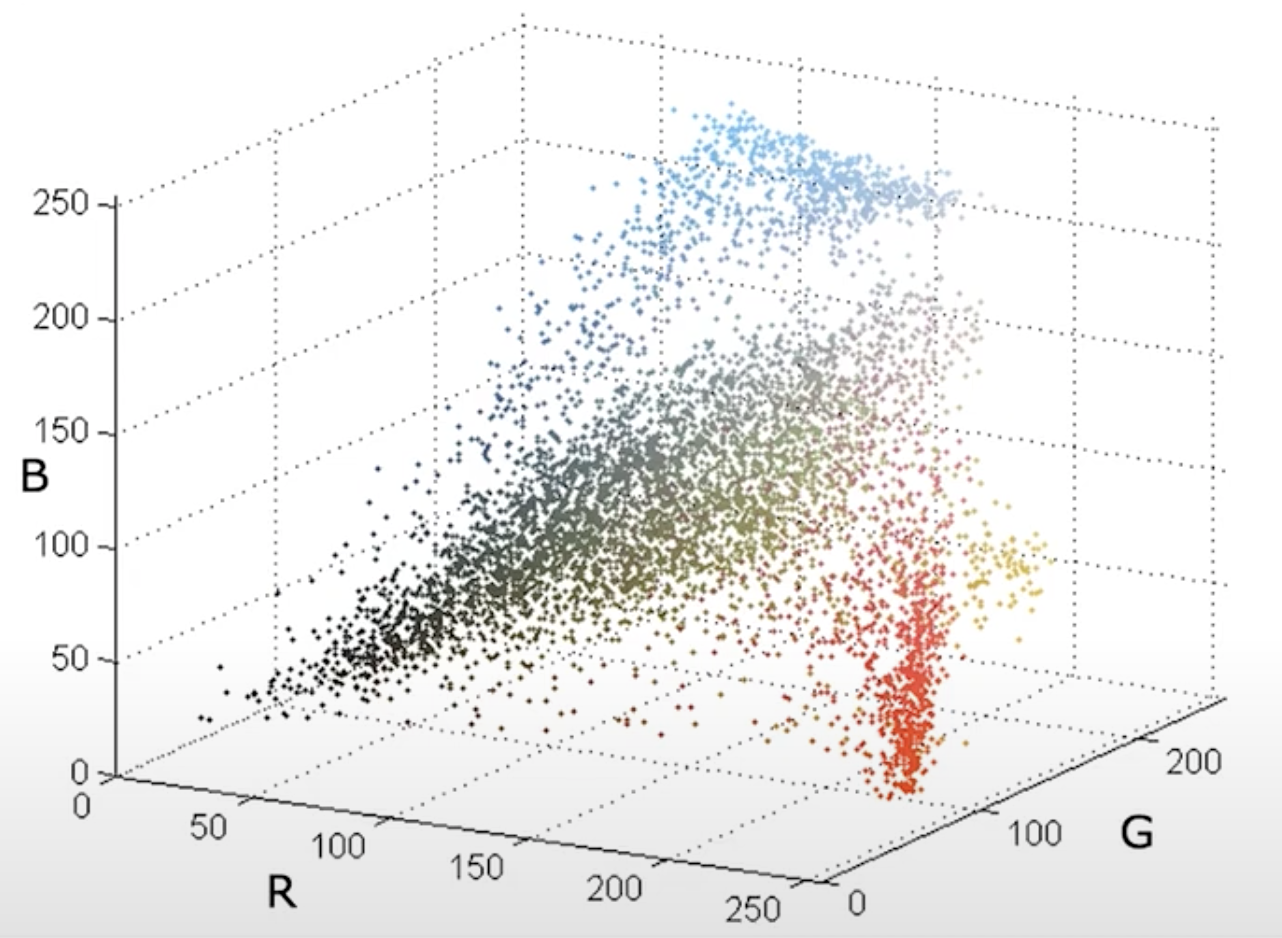
\includegraphics[width=\textwidth]{img/plot-scimmia.png}
         \caption{}
         \label{fig:three sin x}
     \end{subfigure}
        \caption{Le due figure sono un esempio di come un'immagine (a) si possa mappare in un spazio tridimensionale (b) utilizzando come feature i tre canali dell'immagine (RGB).}
        \label{fig:scimmia}
\end{figure}

Una volta completata la mappatura dell'immagine nello spazio scelto, ogni pixel $i$ viene rappresentato con un vettore di feature $f_{i}=[f_{i}^1, f_{i}^2, f_{i}^3, ..., f_{i}^k]$ dove $k$ è il numero di feature scelte. Così come in altri metodi, per guidare l'algoritmo nel raggruppare i pixel, viene utilizzata una misura della loro similarità . In particolare, la similarità viene rappresentata dalla distanza nello spazio dei vettori di feature dei pixel e per calcolarla viene utilizzata quella che è chiamata distanza $L^2$ o distanza euclidea, definita in uno spazio a $k$ dimensioni come:

\begin{equation}
    S(f_{i}, f_{j}) = \sqrt{\sum_{k}{(f_{i}^k-f_{j}^k)^2}}.
\end{equation}

A questo punto, il task della segmentazione è stato totalmente trasformato in un problema di clustering (Figura \ref{fig:scimmia2}) e può essere utilizzato un qualsiasi algoritmo che risolva questo tipo di problema. Di algoritmi che risolvono questo tipo di problema ne esistono diversi, tra i più noti ci sono K-Means e Mean Shift.


\begin{figure}[h!]
     \centering
     \begin{subfigure}[b]{0.4\textwidth}
         \centering
         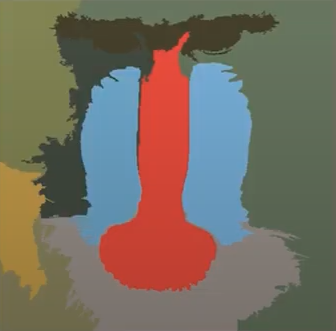
\includegraphics[width=\textwidth]{img/scimmia2.png}
         \caption{}
         \label{fig:y equals x}
     \end{subfigure}
     \hfill
     \begin{subfigure}[b]{0.5\textwidth}
         \centering
         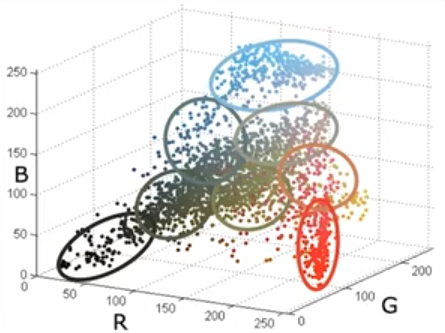
\includegraphics[width=\textwidth]{img/plot-scimmia2.png}
         \caption{}
         \label{fig:three sin x}
     \end{subfigure}
        \caption{Le due immagini mostrano il risultato di un algoritmo di clustering applicato alla mappatura dell'immagine della Figura \ref{fig:scimmia}a. Nella (a) il risultato finale, ovvero l'immagine segmentata; la (b) invece mostra il clusters nello spazio tridimensionale.}
        \label{fig:scimmia2}
\end{figure}




\subsubsection{K-means}
Probabilmente, l'algoritmo di clustering più noto è il \textit{k-means} \cite{lloyd1982least, macqueen1967some}. Il suo funzionamento è abbastanza semplice e si basa sull'obiettivo di trovare il centroide o punto medio, di ogni cluster, ovvero trovare il punto che minimizzi la varianza totale intra-gruppo $Var$, che non è altro che una misura della variabilità all'interno del cluster. Formalmente, il problema è definito come trovare:

\begin{equation}
    \underset{S}{\arg\min} \sum_{i=1}^{k}{|S_{i}| Var(S_{i})}.
\end{equation}

Dove $S={S_{1},S_{2},..., S_{k}}$ è l'insieme dei cluster. Una volta trovati i centroidi di ogni cluster, il cui numero $k$ deve essere definito in anticipo, l'algoritmo classifica ogni punto nello spazio determinando quale dei $k$ centroidi sia il più vicino. Per quanto riguarda la prima fase della ricerca dei centroidi, l'algoritmo parte inizializzando $k$ centroidi e calcolando i cluster secondo la regola del centroide più vicino. A questo punto, l'algoritmo ripete iterativamente questo meccanismo, ricalcolando ogni volta i centroidi dei cluster fino a non convergere, ovvero fino a che i centroidi non cambiano più posizione o comunque il loro cambiamento è sotto una certa soglia.
Ancora una volta purtroppo, le performance di questo algoritmo dipendono fortemente dalla bontà dell'inizializzazione. In questo caso, l'inizializzazione può essere fatta in diverse maniere: la cosa più semplice è quella di inizializzarli randomicamente, ma chiaramente è anche la scelta meno peformante; un altro metodo molto semplice consiste nell'inizializzarli randomicamente, controllando però che nessuno dei centroidi sia molto vicino e in quel caso reinizializzarli; un terzo metodo è quello di scegliere dei centroidi che siano uniformemente distribuiti nello spazio; infine, un ultimo metodo può essere utilizzare il k-means prima su una sottoporzione della distribuzione, e poi utilizzare i centroidi risultanti come inizializzazione per applicare l'algoritmo a tutta la distribuzione.

\begin{figure}[h!]
     \centering
     \begin{subfigure}[b]{0.4\textwidth}
         \centering
         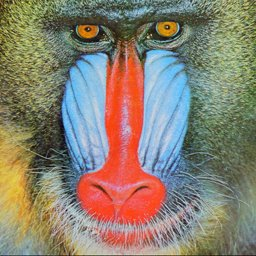
\includegraphics[width=\textwidth]{img/scimmia.jpeg}
         \caption{}
         \label{}
     \end{subfigure}
     \hfill
     \begin{subfigure}[b]{0.4\textwidth}
         \centering
         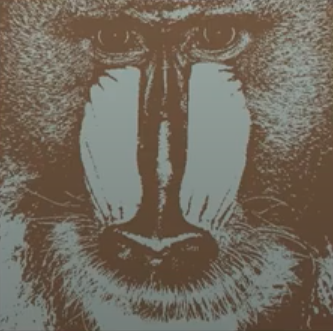
\includegraphics[width=\textwidth]{img/scimmia_k=2.png}
         \caption{}
         \label{}
     \end{subfigure}
     \hfill
     \begin{subfigure}[b]{0.4\textwidth}
         \centering
         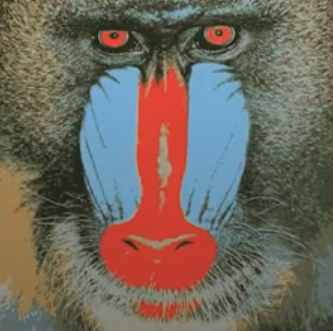
\includegraphics[width=\textwidth]{img/scimmia_k=8.png}
         \caption{}
         \label{}
     \end{subfigure}
     \hfill
     \begin{subfigure}[b]{0.45\textwidth}
         \centering
         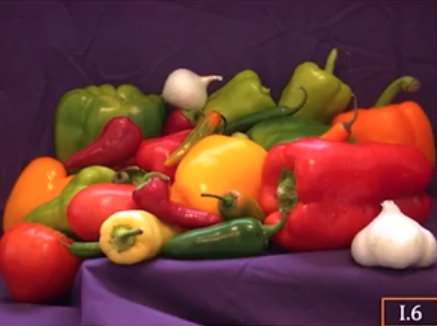
\includegraphics[width=\textwidth]{img/frutta.png}
         \caption{}
         \label{}
     \end{subfigure}
     \hfill
     \begin{subfigure}[b]{0.45\textwidth}
         \centering
         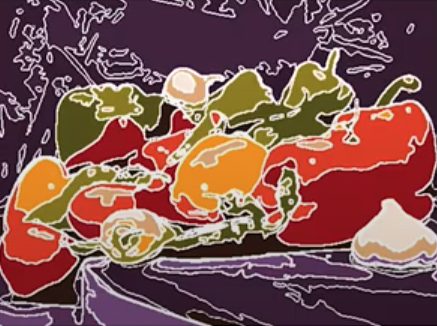
\includegraphics[width=\textwidth]{img/frutta_k=16.png}
         \caption{}
         \label{}
     \end{subfigure}
     \hfill
     \begin{subfigure}[b]{0.45\textwidth}
         \centering
         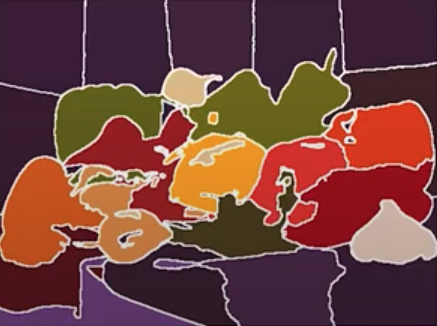
\includegraphics[width=\textwidth]{img/frutta_k=16_xy.png}
         \caption{}
         \label{fig:three sin x}
     \end{subfigure}
        \caption{Le quattro immagini mostrano il risultato dell'algoritmo k-means applicato a immagini RGB: (a) e (d) sono le due imagini originali; (b) mostra il risultato con $k=2$; (c) con $k=8$; (e) è il risultato con $k=16$ e infine (f) è il risultato con $k=16$ ma in uno spazio a cinque dimensioni ovvero $(R,G,B,x,y)$ dove $x$ e $y$ rappresentano le coordinate dei pixel nell'immagine, mentre per tutte le altre è stato utilizzato uno spazio a tre dimensioni ovvero $(R,G,B)$.}
        \label{fig:scimmia_frutta}
\end{figure}






\subsubsection{Mean Shift}
Come detto nel paragrafo precedente, l'algoritmo k-mean ha lo svantaggio di essere molto sensibile rispetto all'inizializzazione dei centroidi. Inoltre, un altro svantaggio del k-mean è che l'utente deve decidere a priori il numero di cluster. L'algoritmo \textit{mean shift} \cite{fukunaga1975estimation, comaniciu_mean} cerca di mitigare questi due problemi. Anche mean shift è un algoritmo iterativo e in particolare, il meccanismo generale si basa sul trovare le mode della distribuzione dei punti nello spazio, che ad alto livello possono essere pensate come i punti dove la distribuzione è più densa. Il funzionamento dell'algoritmo è il seguente: per ogni punto seleziona intorno a questo una finestra di dimensione $W$, che è l'unico parametro dell'algoritmo, e successivamente calcola la moda della distribuzione dei punti all'interno di quella finestra, che sarà il centro della finestra all'iterazione successiva. Ripetendo questo meccanismo finché il vettore di spostamento della moda, ovvero la distanza della moda di un' iterazione a quella dell'iterazione successiva, non si azzeri oppure non scenda sotto una certa soglia, l'algoritmo trova la moda verso la quale il punto di partenza è stato "attratto". Infine, il mean shift crea i cluster trovando i "bacini di attrazione", ovvero gli insiemi di punti che vengono attratti verso la stessa moda. La Figura \ref{fig:scimmia_frutta} mostra alcuni esempi dell'applicazione del mean shift.




\subsection{Algoritmi Supervised}
In generale, come già menzionato, una volta mappata l'immagine in uno spazio multidimensionale di feature, il task della segmentazione si può ricondurre, nel caso in cui il numero di classi fosse noto a priori, in un classico task di classificazione Machine Learning. Di conseguenza, tutti gli algoritmi  di Machine Learning per la classificazione diventano validi per risolvere il problema della segmentazione. Di algoritmi di classificazione ne esistono svariati e tra i più popolari vi sono l'SVM (Support Vector Machines), il Regressore logistico, alberi decisionali, K-nearest neighbor e molti altri. La principale differenza con gli algoritmi menzionati nei paragrafi precedenti (\ref{metodi_soglia}, \ref{metodi_dividi_fondi}, \ref{metodi_grafi}, \ref{metodi_contorni}, \ref{metodi_clustering}) è che questi ultimi rientrano nella categoria di algoritmi unsupervised, mentre tutti i classificatori di Machine Learning appena menzionati rientrano in quella supervised, ovvero hanno bisogno di un dataset per poter apprendere i propri parametri e riuscire a classificare.

%\subsubsection{Support Vector Machines}
%FORSE DA TOGLIERE

%L'SVM è un algoritmo di classificazione il cui obiettivo è quello di costruire un classificatore binario lineare che riesca a separare l'insieme di punti, che gli sono stati forniti sotto forma di dataset, nelle due classi. Il classificatore lineare che viene costruito è definito dalla seguente equazione:

%\begin{equation}
%    y=W^{T}X+b.
%\end{equation}

%dove $W$ e $b$ sono i parametri del classificatori che vengono appresi durante algoritmo, $X$ è il vettore in input e $y$ rappresenta il valore con cui il classificatore deciderà la label di $X$. L'idea generale dietro l'SVM è quella di costruire un iperpiano di forma

%\begin{equation}
%    W^{T}X+b=0.
%\end{equation}

%che massimizzi la sua distanza dai punti del dataset rimanendo però coerente con il dataset, ovvero che clasifici bene i suoi punti. in particolare, per quanto riguarda questa distanza, durante le iterazioni alcuni punti, chiamati vettori di supporto (\textit{support vectors}, da cui il nome) assumono un'importanza più elevata perché i più vicini al iperpiano. In particolare, questa distanza rappresenta la distanza tra l'iperpiano del classificatore, anche chiamato confine di decisione, e i due iperpiani paralleli che intersecano i vettori di supporto delle due classi.




\section{Approcci di Deep Learning}
Oltre agli approcci classici, vi sono tecniche di Deep Learning che utilizzano architetture complesse, per riuscire ad apprendere il pattern d'interesse e in particolare, per apprendere le feature che determinano la semantica dei pixel, cosa che invece deve essere fatta manualmente quando si utilizzano gli algoritmi di Machine Learning (fase della \textit{feature extraction}).\\

%\subsection{Architetture di Deep Learning}

 
 \subsection{Architetture basate sul contesto}
 \label{context_based}
Questa categoria di architetture utilizza una tipologia di informazione molto importante e che i metodi di cui abbiamo parlato nei capitoli precedenti non utilizzano, ovvero il contesto di un pixel. In particolare, il contesto risulta molto importante per la classificazione semantica di un pixel, in quanto spesso le feature locali di un pixel come il colore, la luminosità, ma anche altre più complesse, non sono sufficienti per distinguere due pixel di classi diverse. Come già visto, in generale nel campo della Computer Vision la tipolgia di architettura più utilizzata è la CNN, che si basa sulle presenza di strati convoluzioni, ed è proprio grazie a questi che l'architettura riesce ad estrapolare il contesto di un pixel. In particolare, la categoria delle architetture context-based fa un forte uso delle convoluzioni in diverse forme. Una delle varianti più utilizzate per catturare un contesto più ampio del pixel, senza però andare ad aumentare di troppo il costo computazionale, è la convoluzione dilatata. In particolare alcune, per fare in modo di costruire campi ricettivi con diverse ampiezze, fanno uso delle convoluzioni dilatate a diverse scale. Ad esempio, la DilatedNet \cite{yu2015multi} fa uso di cinque diversi parametri di dilatazione, ovvero 1,2,4,8 e 16, ottendeno una mIoU del 67.6\% sul dataset PASCAL VOC 2012. In \cite{parsenet} le feature locali di un pixel vengono fuse con le feature globali dell'immagine, così facendo aggiungono al contesto locale del pixel quello globale, ottenendo una mIoU di 69.8\% sul PASCAL VOC 2012. In \cite{pspnet} invece, viene utilizzato un modulo chiamato \textit{Pyramid Pooling Module} (PPM), che utilizza uno strato di pooling a diverse scale per poi fondere i risultati di questi pooling insieme, in modo da avere informazioni di contesto a diverse scale (Figura \ref{fig:PPM}). In particolare, l'idea è che con il solo utilizzo del contesto globale, si ha una perdita di informazioni nelle sotto regioni, mentre utilizzando il PPM vengono catturate le informazioni a diverse scale, compresa quella globale. Il PPM ha poi ispirato moltri altri lavori che, apportando modifiche, hanno migliorato ancora di più le performance, come ad esempio la DeepLabV2 \cite{deeplabv2}, che  a partire dall'idea del PPM ha costruito il modulo Atrous Spatial Pyramid Pooling (ASPP), sostituendo in sostanza la normale convoluzione e il pooling con la convoluzione dilatata a diverse scale, ovvero con diverse dilatazioni, ottenendo su PASCAL VOC una mIoU di 79.7\%.

\begin{figure}[h!]
    \centering
    \hspace*{-0.1in}
    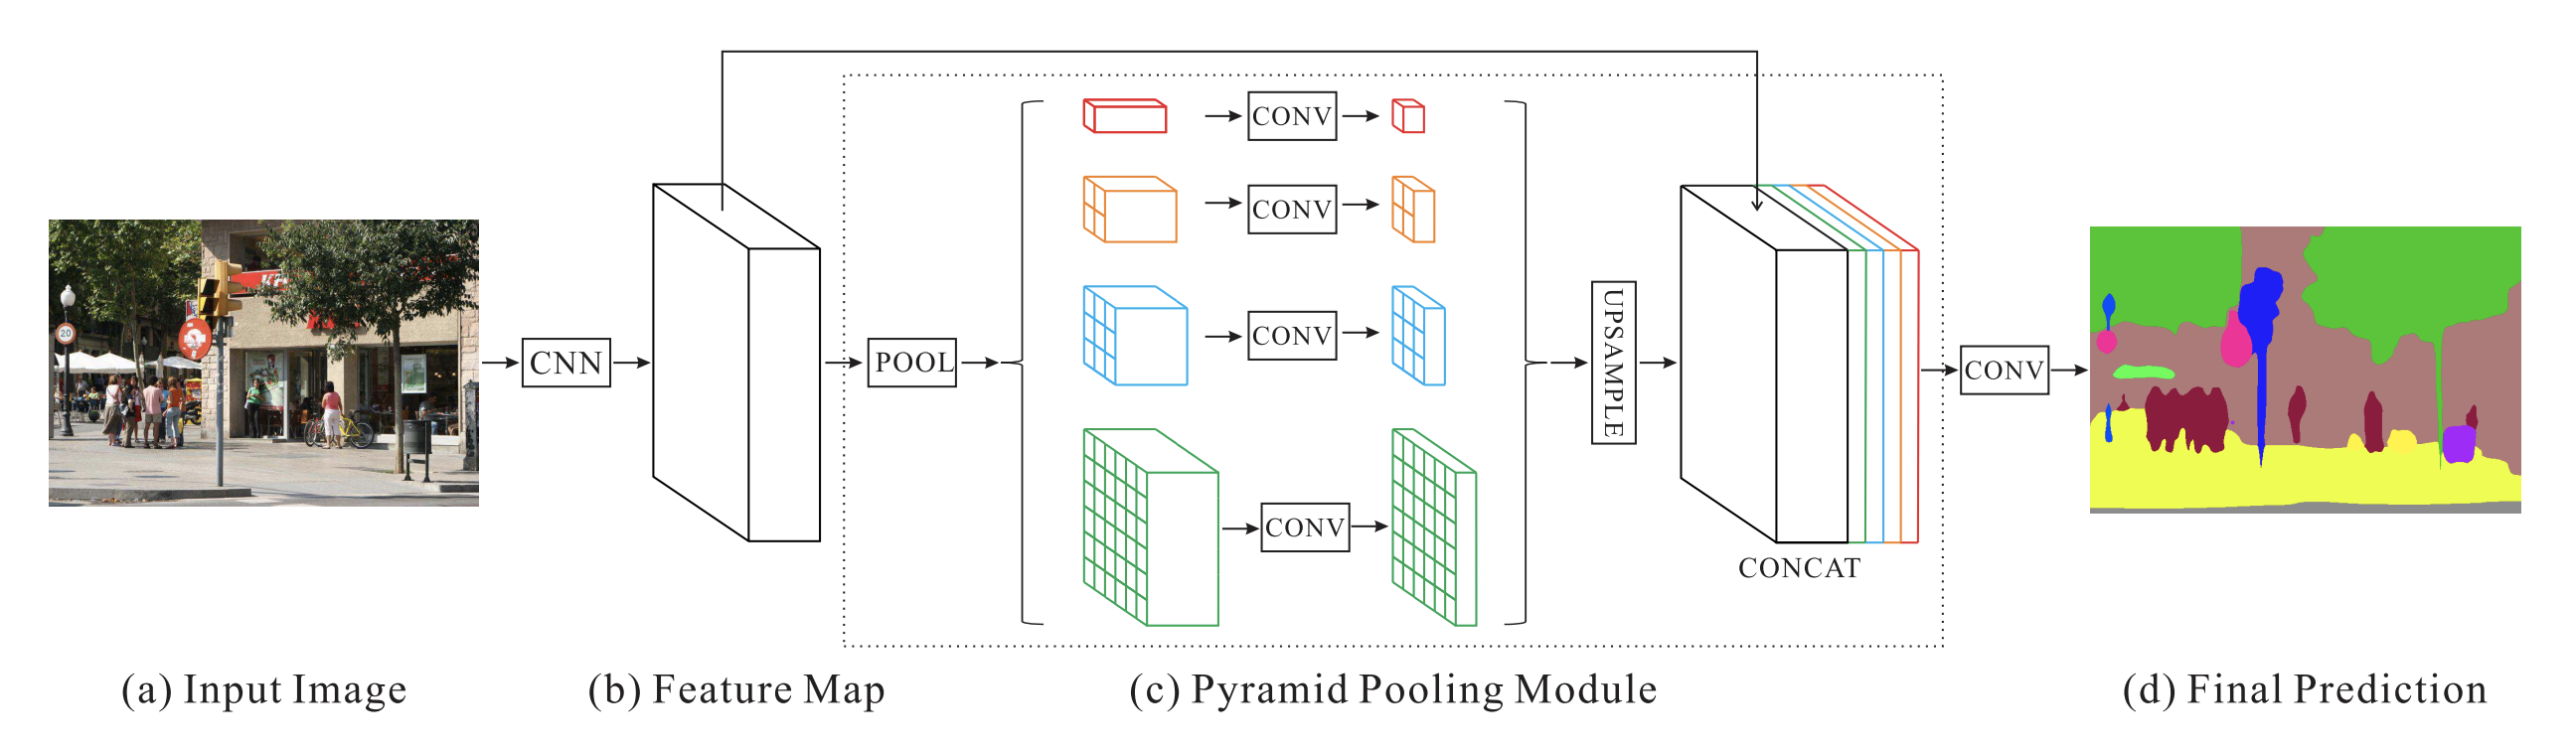
\includegraphics[scale=0.3]{img/PPM.png}
    \caption{Illustrazione del Pyramid Pooling Module (PPM) \cite{pspnet}.}
    \label{fig:PPM}
\end{figure}




 
 \subsection{Architetture basate sul feature-enhacement}
Il concetto generale alla base di questa categoria di architettura è che, nelle CNN, l'estrazione strato per strato di feature sempre più di alto livello causa una perdita di informazioni spaziali. In particolare, a causa soprattutto del pooling e delle convoluzioni con stride, le feature avanzando progressivamente nella rete, diminuiscono di risoluzione e di conseguenza perdono le informazioni spaziali, che in task come la classificazione non sono importanti, ma che invece lo sono nel task della segmentazione. La soluzione proposta da questa categoria di architetture per risolvere questo problema è unire i due aspetti, ovvero unire le feature dei primi livelli, che hanno soprattutto informazioni spaziali, con quelle dei livelli più profondi, che invece non hanno molta informazione spaziale ma contengono informazioni sulle feature di alto livello. Una delle prime architteture di questo tipo è stata la FCN \cite{FCNs}, che mette in atto questa idea aggiungendo delle \textit{skip connections}, collegando così le feature degli strati intermedi con quelle degli ultimi strati. La UNet \cite{unet} è un'altra architettura che si rifà a questo concetto ed è una delle architetture più note nel campo della segmentazione semantica. In particolare, la UNet, chiamata così per la sua peculiare forma a U, a differenza della FCN utilizza delle skip connections tra tutti gli strati, ovvero connette tutte le feature della prima parte della rete, responsabile della feature extraction e chiamata encoder, a quelle della seconda parte della rete, chiamata decoder (Figura \ref{fig:unet}).
 
 \begin{figure}[h!]
    \centering
    \hspace*{0.1in}
    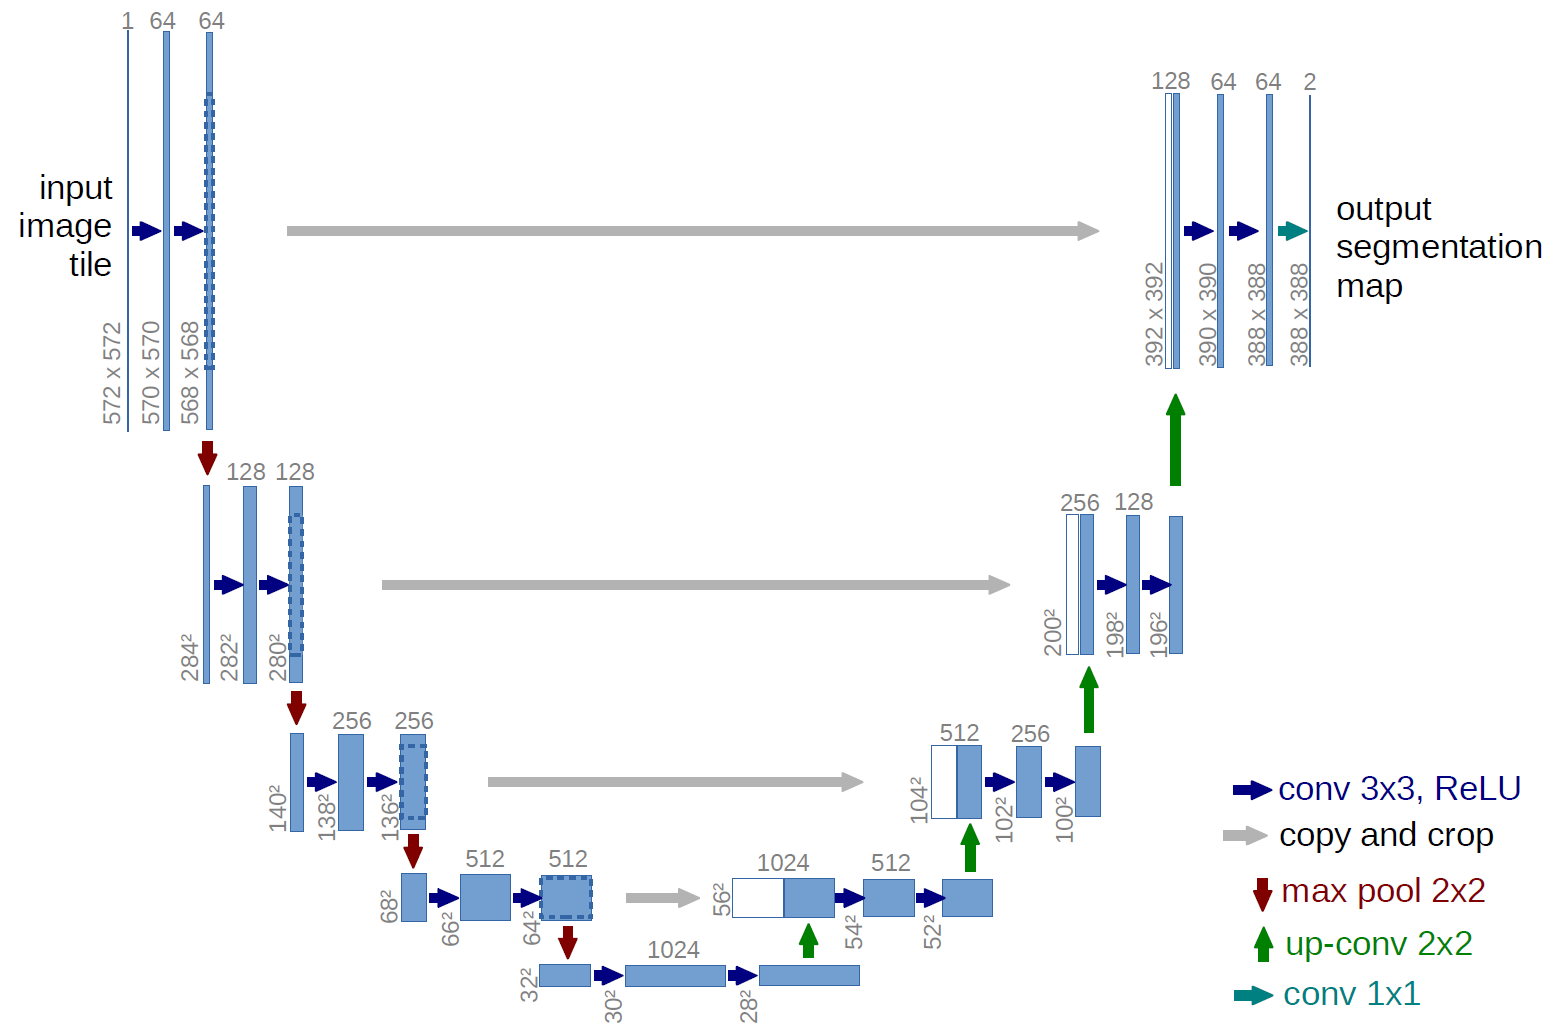
\includegraphics[scale=0.22]{img/unet.png}
    \caption{Architettura della UNet \cite{unet}.}
    \label{fig:unet}
\end{figure}
 
 
\subsection{Architetture basate sulla deconvoluzione}
La prima architettura di questo tipo è stata la DeconvNet \cite{deconvnet}, che ha una struttura encoder-decoder. In particolare, questa rete utilizza, a parte i classici moduli di pooling, convoluzione, e via dicendo, altre due tipologie di modulo, ovvero l'unpooling e la deconvoluzione. L'idea alla base del loro utilizzo è far fronte al problema della perdita di precisione nelle informazioni spaziali, nella parte di decoder in cui viene fatto l'upsample delle feature map per riportarle alla risoluzione originale. In particolare, negli strati di pooling dell'encoder, viene memorizzato l'indice della cella più grande, in modo che, nella fase di upsample, il modulo di unpooling possa ricreare la stessa finestra che era passata dentro lo strato di pooling. L'output dell'unpooling, tuttavia, ha delle celle azzerate, questo poiché nel corrispettivo pooling nell'encoder viene memorizzata soltanto la cella maggiore, ma non le altre. Per risolvere questo problema l'output del modulo di unpooling viene passato alla deconvoluzione che, grazie ai parametri appresi, riesce a ricostruire la feature map (Figura \ref{fig:deconv}).
 
\begin{figure}[h!]
    \centering
    \hspace*{0.1in}
    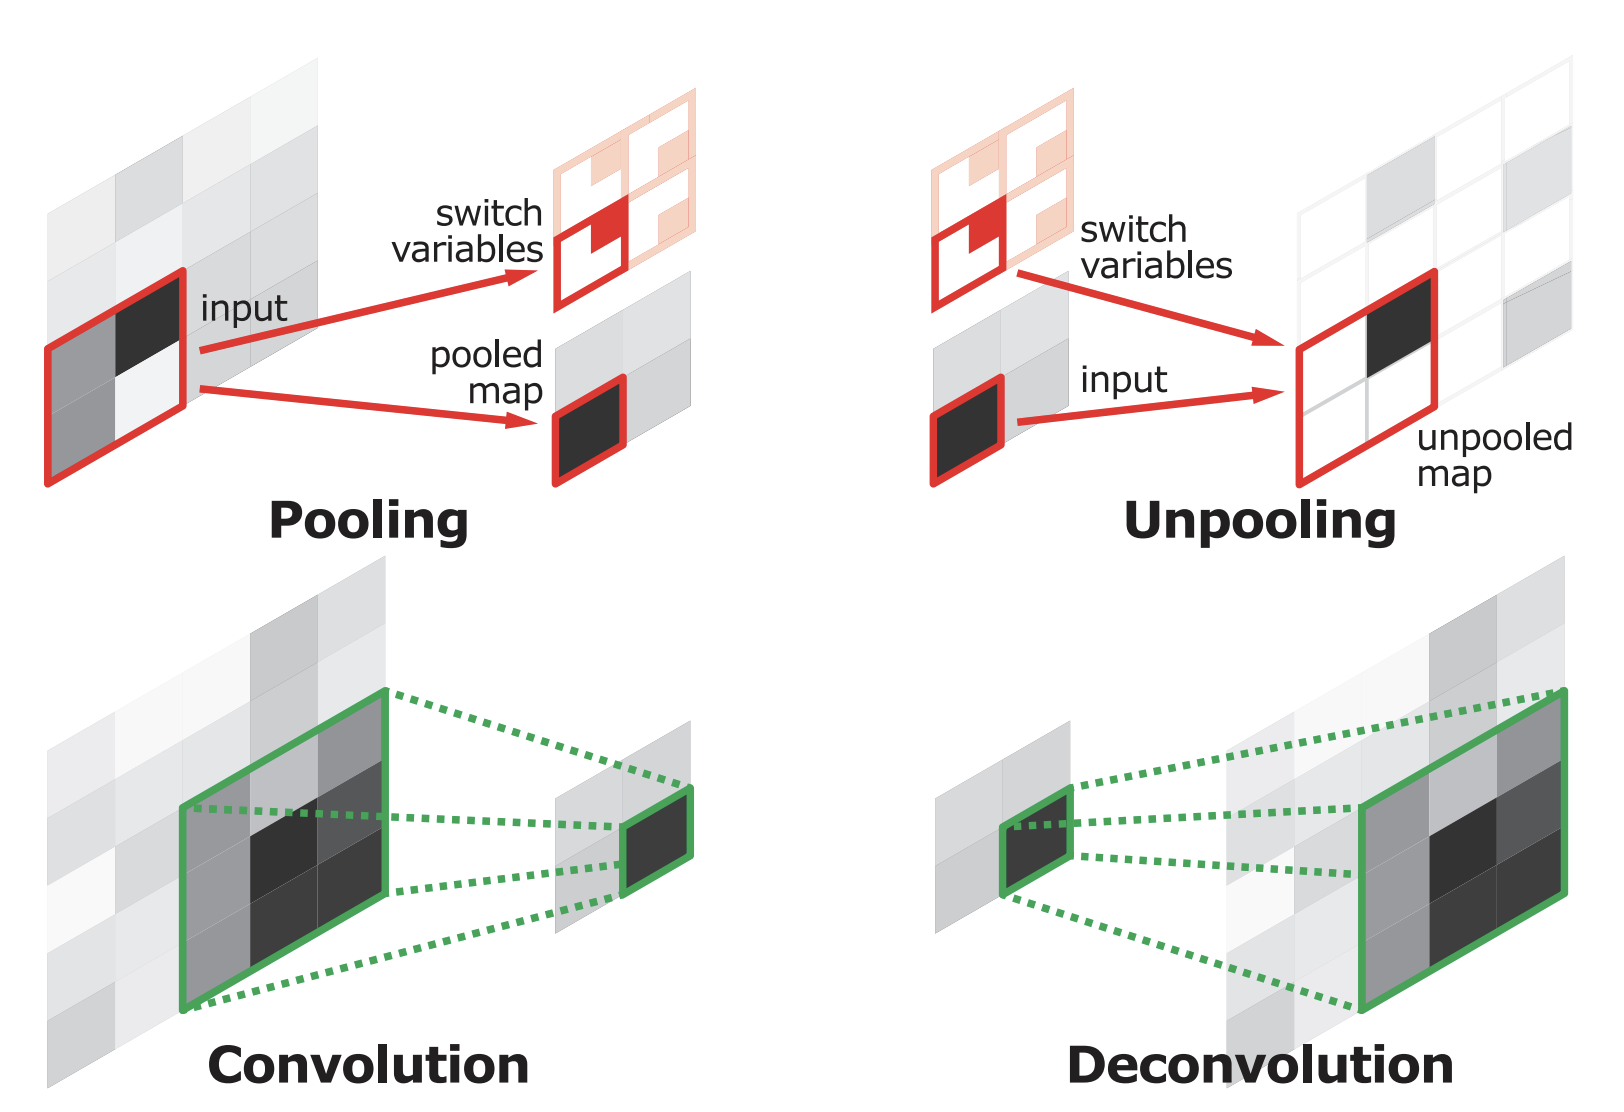
\includegraphics[scale=0.35]{img/deconv.png}
    \caption{Illustrazione dei due moduli di unpooling e di deconvoluzione \cite{deconvnet} e della loro differenza con, rispettivamente, il pooling e la convoluzione.}
    \label{fig:deconv}
\end{figure}
 
 

 
\subsection{Architetture basate sulle GAN}
Questa tipologia di architettura è composta da due reti chiamate "segmentatore" e "rete avversaria" (\textit{adversarial network}). La prima ha la responsabilità, partendo dall'immagine in input, di crearne una partizione in sotto-regioni non intersecanti, ovvero la maschera. La seconda, invece, ha la responsabilità di distinguere tra l'output della prima rete e la maschera corretta. In particolare, le due reti sono messe una contro l'altra: il segmentatore ha l'obiettivo di non far capire alla seconda rete la differenza tra il suo output e la vera maschera, mentre la seconda rete (Figura \ref{fig:anet}) ha l'obiettivo di capire la differenza. L'ANet \cite{anet} è una delle prime reti di questo tipo utilizzate per la segmentazione semantica e in particolare, il concetto principale alla sua base è che la rete avversaria, a differenza di una classica loss function utilizzata per l'addestramento di una rete, riesce a cogliere differenze di più alto livello tra l'output del segmentatore e la maschera, come ad esempio differenze nella forma degli oggetti o nelle loro proporzioni. La prima rete, quella responsabile della segmentazione, utilizza per l'addestramento una loss function composta, ovvero la loss function finale è il risultato della somma pesata di due ulteriori loss function, una classica cross entropy e un'adversarial loss function. In particolare, la seconda loss function rappresenta quanto la rete avversaria riesca a distinguere tra il suo output e la maschera corretta.
 

\begin{figure}[h!]
    \centering
    \hspace*{0in}
    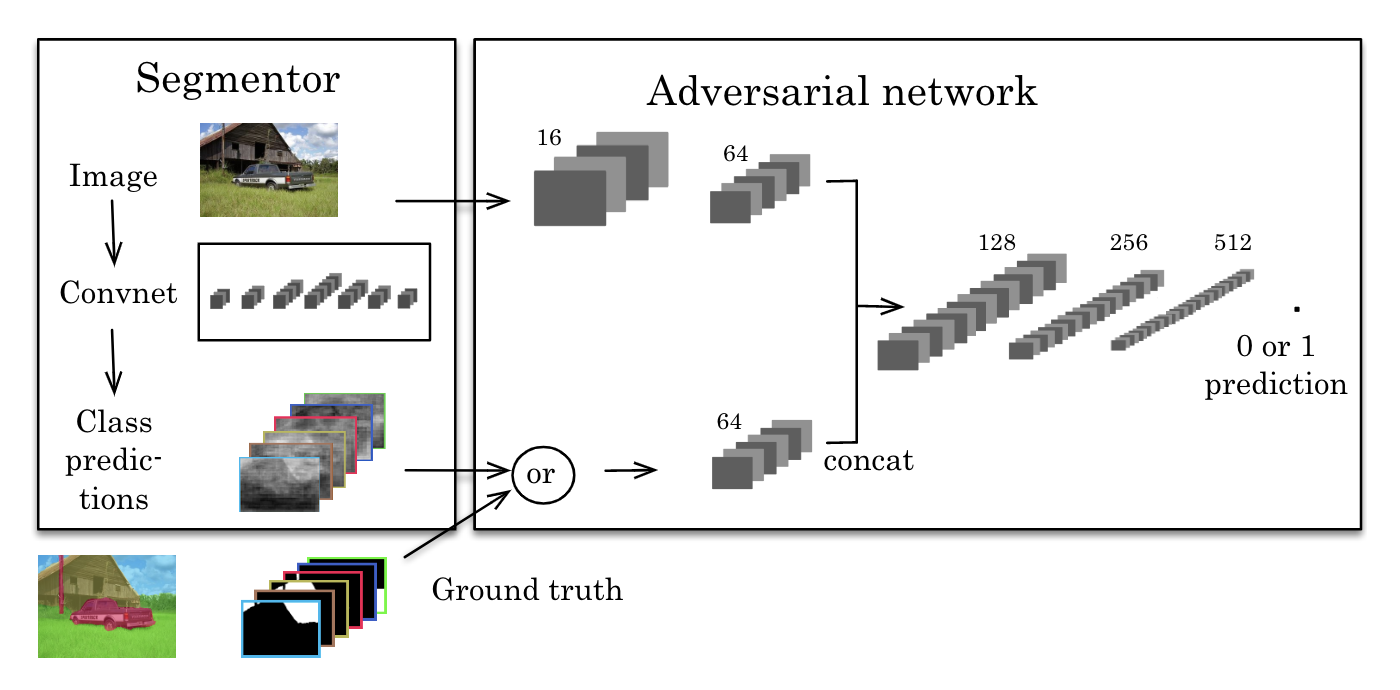
\includegraphics[scale=0.55]{img/gan.png}
    \caption{Panoramica dell'architettura basata sulle GAN proposta in \cite{anet}. A sinistra il segmentatore prende l'immagine RGB come input, e produce la maschera. A destra la rete avversaria prende la maschera prodotta dal segmentatore e produce una label (1 = maschera corretta, o 0 = maschera sintetica del segmentatore). La rete avversaria opzionalmente può prendere anche l'immagine RGB come input.}
    \label{fig:anet}
\end{figure}

